\documentclass[10pt,notitlepage]{article}
\usepackage[utf8]{inputenc}
\usepackage[english]{babel}
\usepackage{amsmath}
\usepackage{amsfonts}
\usepackage{amssymb}
\usepackage{hyperref}
\usepackage{graphicx}
\usepackage{listings}
\usepackage{lmodern}
\usepackage{hyperref}
\usepackage{float}
\usepackage[left=2cm,right=2cm,top=2cm,bottom=2cm]{geometry}
\author{Dylan Geyer}
\title{Turnigy Talon Hexcopter v2.0 Build}
\begin{document}
\maketitle
\section{Intro}
This document details how the Turnigy Talon Hexcopter v2.0 was assembled and the peripheral devices were mounted so that others may replicate this process. It first details assembling the frame, and then mounting each peripheral device (motors, ESC's, Odroid-XU4, etc..).

\section{Turnigy Talon Hexcopter v2.0 Frame}
This first section will detail how the carbon fiber frame is put together.

\subsection{Bolts}
The first thing to do is make sure you know which screws correspond to each label in the figures that will follow. 

\begin{figure}[H]
	\centering
	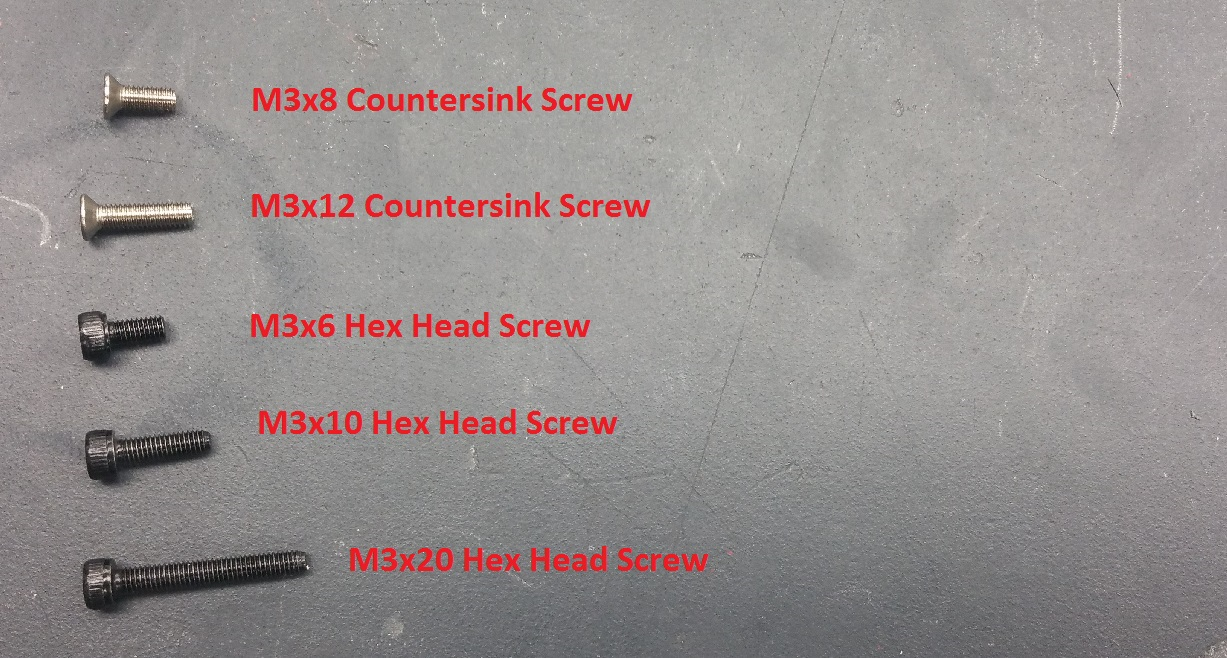
\includegraphics[width=\textwidth]{Images/Bolts2.jpg}
	\caption{Bolt definitions.}
\end{figure}

\begin{figure}[H]
	\centering
	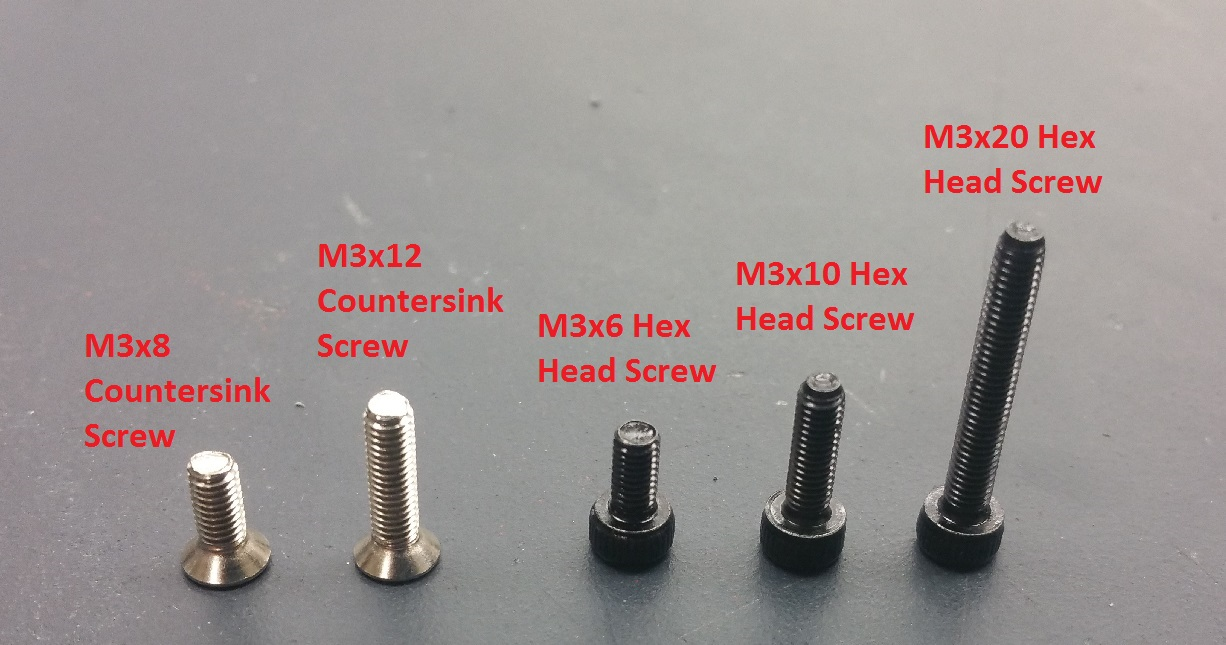
\includegraphics[width=\textwidth]{Images/Bolts1.jpg}
	\caption{Another view of the bolts.}
\end{figure}

\subsection{Arm}
Now that there is a quick reference guide for each of the types of screw, we can begin building the frame. The first part to be constructed is the motor mount and the tip of each arm.

\begin{figure}[H]
	\centering
	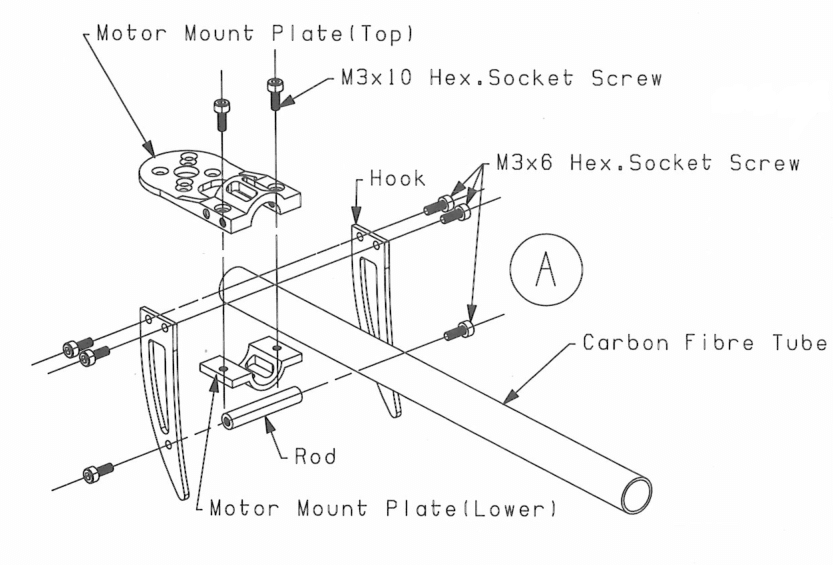
\includegraphics[width=\textwidth]{Images/ArmOuter.png}
	\caption{Instructions for assembling motor mount.}
\end{figure}
After carefully following the directions above we are left with a carbon fiber tube with an assembled motor mount which is shown in the image below.

\begin{figure}[H]
	\centering
	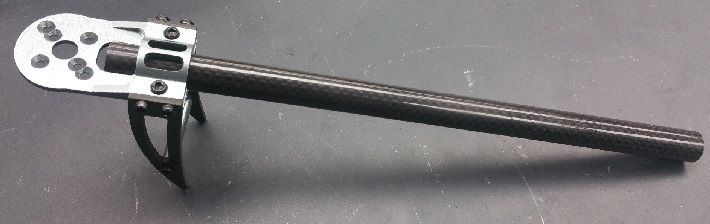
\includegraphics[width=\textwidth]{Images/MyArm.jpg}
	\caption{My completed motor mount.}
\end{figure}

\subsubsection{Frame Mount}
Now that the motor mount has been attached to one end of the carbon fiber arm, it is time to attach the frame mount to the other end so that the center plates will be able to hold each arm in place.
\begin{figure}[H]
	\centering
	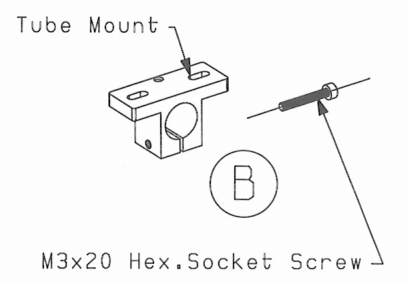
\includegraphics{Images/ArmInner.png}
\end{figure}

\subsection{Center Support}
Once all of the arms have been assembled they must be affixed to the top and bottom plates to keep everything stable. This step is a bit tricky as each arm must be loosely connected to the top and bottom plates before tightening the screws down or it will be impossible to insert the other arms.

\begin{figure}[H]
	\centering
	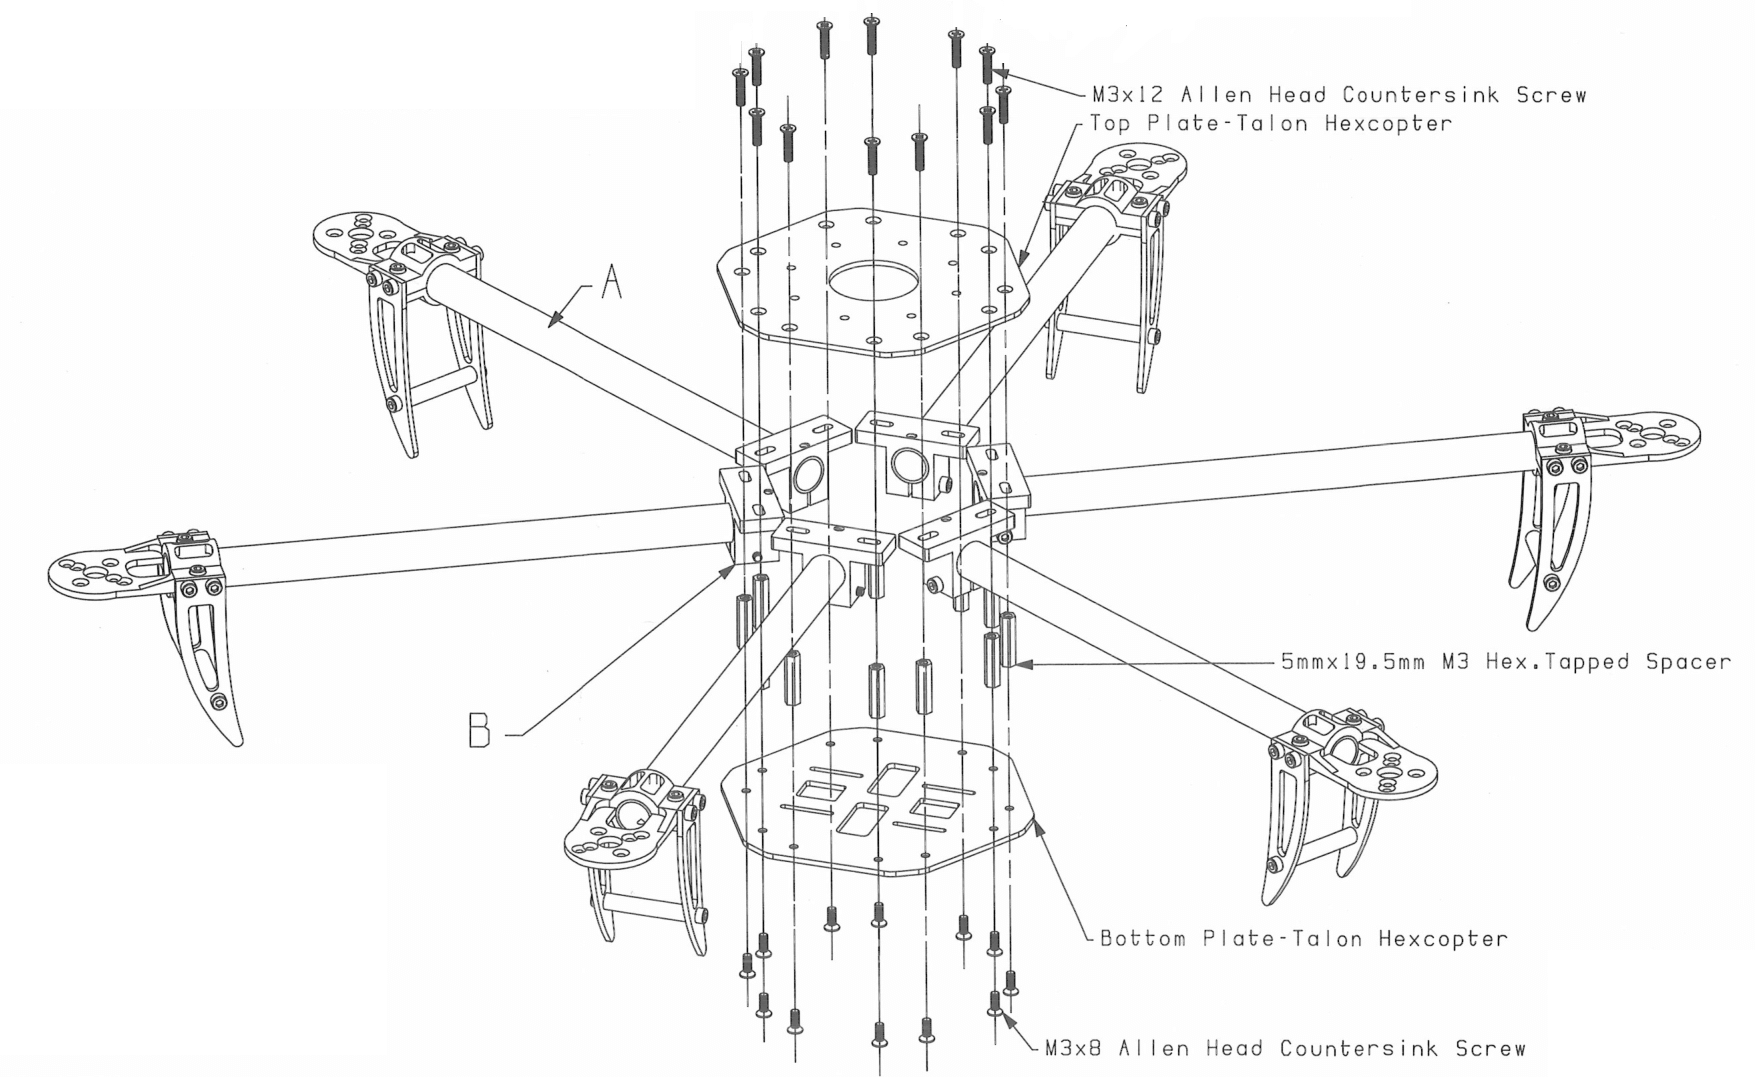
\includegraphics[width=\textwidth]{Images/CenterConsole.png}
	\caption{Instructions for Top/Bottom plates.}
\end{figure}

\section{Motors}
Once the whole frame has been constructed it is time to attach the DC motors. These DC motors will attach to the very tip of the each arm with their power cables routing through the hollow carbon fiber arms.
\subsection{Mounting}
One note for this particular build is that the leads that came attached to the motor were much too short to connect to the controllers in the center console. This was fixed by simply soldering some 16 gauge extension wires onto the motor leads and then connecting these to the ESC's. 
\subsection{Electronic Speed Controllers}
ESC's are attached to the DC motor leads \textbf{after} they come out of the arm holes and are in the center console.

\section{Controllers}
\subsection{ODROID-XU4}
\subsection{Pixhawk}
\subsection{Power Distribution Board}

\section{Camera}


\end{document}